\documentclass[10pt, a4paper]{article}
%%%%%%%%%%%%%%%%%%%  Global Defines  %%%%%%%%%%%%%%%%%%%%%
\usepackage[utf8]{inputenc}
\usepackage[english]{babel}
\usepackage[document]{ragged2e}
\usepackage{indentfirst}
\usepackage{amsmath}
\usepackage{url}
\usepackage{graphicx}
\graphicspath{{res/}}
\usepackage{subcaption}
%\usepackage{natbib}
\usepackage{multicol}
\usepackage{geometry}
\usepackage{wrapfig}
\usepackage{lipsum}

%\geometry{legalpaper, landscape, margin=2in}
\geometry{legalpaper, margin=0.7in}

%%%%%%%%%%%%%%%%%%%  Fonts  %%%%%%%%%%%%%%%%%%%%%%%%%%
% https://tug.org/FontCatalogue/sansseriffonts.html
%\usepackage{courier} 

%\usepackage{helvet} %arial
%\renewcommand{\familydefault}{\sfdefault}

%\usepackage{times}

%\usepackage{tgadventor}
%\renewcommand*\familydefault{\sfdefault} %% Only if the base font of the document is to be sans serif
%\usepackage[T1]{fontenc}

%%%%%%%%%%%%%%%%%%%  Title Define  %%%%%%%%%%%%%%%%%%%%%%%%
\title{Pedestrian segmentation based on U-net.}
%\date{2020/11/09}
\date{}
\author{Tom Hanks \\ Student ID: xxxxxxxxx}

%%%%%%%%%%%%%%%%%%%  Body begin  %%%%%%%%%%%%%%%%%%%%%%%%
\begin{document}
	\pagenumbering{gobble}
	\maketitle
	%\newpage
	\pagenumbering{arabic}
 	
	\begin{multicols}{2}
%%%%%%%%%%%%%%%%%%%  Abstract  %%%%%%%%%%%%%%%%%%%%%%%%%%
	\begin{abstract} \justify %abstract
Image segmentation is a basic task of computer vision for image recognition and understanding. It’s the pre-program for recognizing and understanding an image. The effect of image segmentation is self-evident for understanding the image. The accuracy and effectiveness of image segmentation are of great significance to the development of intelligent computer vision. This article will review some commonly used and popular image segmentation algorithms and will show pedestrian segmentation experiments project based on U-Net. Project source code available at my github channel\footnote{\label{}\url{https://github.com/StevenHuang2020/Pedestrian-Segmentation}}.
	\end{abstract}

%%%%%%%%%%%%%%%%%%%  Section 1 Literature review  %%%%%%%%%%%%%%%%%%%%%%%%%%
	\setlength{\lineskip}{3em}     % line space
	\setlength{\parskip}{0.5em}     % paragraph space
	%\linespread{4.2}

	\section{Literature review} \justify
	%\setlength{\leftskip}{3cm}
	%\setlength{\parindent}{5ex}   	
	Earlier image segmentation algorithms were general based on cognition and basic knowledge on the pixel level, which is the similarity of pixels within objects and the dissimilarity of object boundaries. These common algorithms include thresholding, edge detection-based methods, Region Growing, Split and merge methods. The classic thresholding algorithm for two-segment, Otsu's algorithm is to exhaust the appropriate threshold based on statistical indicators, so that the internal pixel distance of the two parts of the segmentation is the smallest, and the distance between the two parts is the largest \cite{otsu1979threshold}. The edge detection-based algorithm always relies on the clear boundary between the objects in the image and the boundary line that can be connected. These traditional methods can perform well only on very simple tasks or special condition images and are difficult to competent for general image segmentation tasks.
	\par 	
	%\setlength{\parindent}{5ex}   
	Many machine learning (ML) algorithms are more versatile and accurate than previous traditional algorithms, often used for image segmentation. Image segmentation can be regarded as a classification problem, and the goal is to classify different pixels in one image into classes belonging to different objects. It should be noted that the classification model requires some labelled samples to learn the appropriate parameters for effective object segmentation. Numerous classification models such as Decision Tree (DT), Logistic regression, Support Vector Machines (SVM), Multi-layer Perceptron (MLP), etc. are all applied to various classification tasks \cite{pedregosa2011scikit}. Liu et al. \cite{liu2006region} proposed a decision tree based semantic segmentation image retrieval system, which optimizes the tree pruning process and improves performance. Mizushima and Lu \cite{mizushima2013image} demonstrated an effective algorithm for classifying and grading apples using image segmentation based on SVM and Otsu’s thresholding method, with an error rate less than 2 percent. On the other hand, the clustering model can be selected to do image segmentation tasks when there are no labeled samples. Common clustering algorithms include K-Means, Agglomerative clustering, DBSCAN, OPTICS, etc. The fastest, simplest and efficient K-Means algorithm, due to its linear time complexity, is particularly suitable for clustering large-scale data sets. However, the clustering numbers parameters required by this algorithm must be determined through accurate measurements. Ray and Turi \cite{ray1999determination} proposed an algorithm based on distance measurement within and between clusters, which can automatically calculate the number of clusters.
	\par
	Due to its high accuracy and strong versatility, Deep learning is the current new generation algorithms for generic image segmentation. Unlike the previous algorithms are basically based on the pixel level, the deep learning algorithm performs image segmentation rely on automatically extracted semantic features, which significantly increases robustness and accuracy. According to the research of Minaee et al. \cite{minaee2020image}, the current classic CNN models for semantic segmentation include fully convolutional network (FCN), SegNet, U-Net, V-net, etc. The end-to-end fully convolutional network FCN obtains good segmentation results on the PASCAL VOC data set by changing the fully connected layer in the current excellent image classification neural network \cite{long2015fully}. Noh et al. \cite{noh2015learning} proposed a convolutional network based on Encoder-Decoder that includes transpose convolution and unpooling layers, which alleviates the limitations of FCN. The other encoder-decoder model, the Segnet, which directly uses the pooling indices of the previous max-pooling layer in the encode upsampling stage, thereby effectively reducing the inference time\cite{badrinarayanan2017segnet}. Ronneberger, et al. \cite{ronneberger2015u} proposed the U-Net model inspired by the previous FCN and encoder-decoder architecture model and achieved good performance on the medical image segmentation task. Milletari et al. \cite{milletari2016v} proposed V-net, a fully CNN model based on U-net and successfully segment 3D MRI prostate medical images. 

%%%%%%%%%%%%%%%%%%%  Section 2 U-net Model %%%%%%%%%%%%%%%%%%%%%%%%%
	\section{U-net Model} \justify
	\begin{figure*} %[htb] %[h!]
        \centering
	  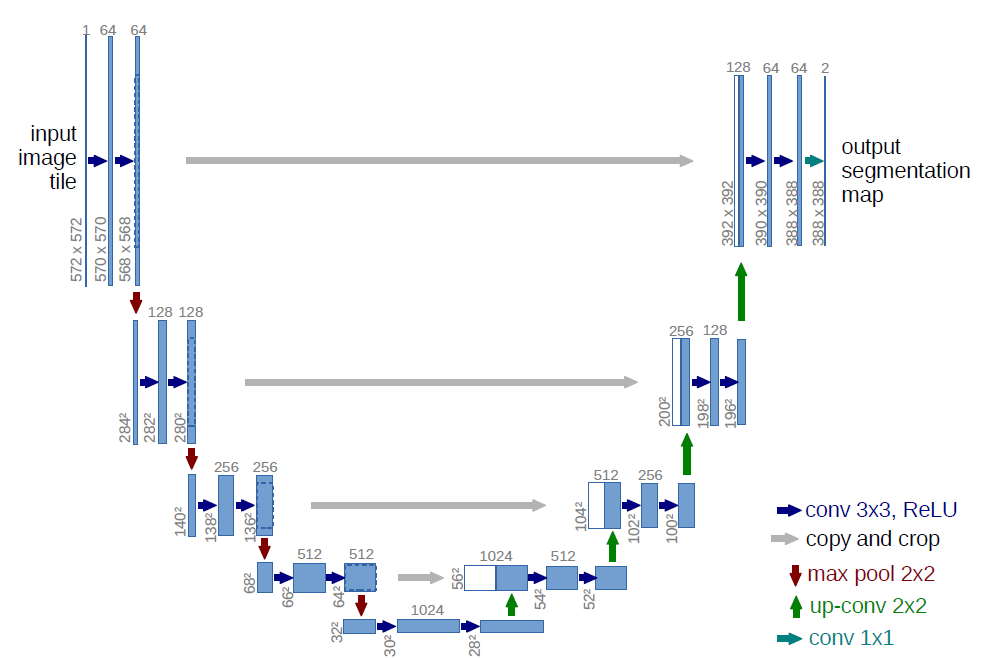
\includegraphics[width=0.5\linewidth]{Capture.PNG}
	  \caption{U-Net Architecture \cite{ronneberger2015u}.}
	  \label{fig:Unet}
	\end{figure*}

	The experiment model is borrowed from the U-Net model and the architecture of the U-Net model is shown in Figure \ref{fig:Unet}. The input of the model is modified to 255x255x1, and the output is a segmentation mask image of the same size. The model uses only convolutional layers and removes fully connected layers and uses convolution and deconvolution layers at different scales to increase the ability to recognize objects of different scales. The last convolutional layer uses sigmoid as the activation function. The loss function uses Dice loss which defined as follows,
	%\begin{footnotesize} %tiny scriptsize footnotesize small normalsize large Large LARGE huge Huge
	\begin{equation}
	\begin{aligned}
	Loss(y_{true}, y_{pred}) = \\1 - \frac{2\sum_{pixels}y_{true}y_{pred} + smooth }{\sum_{pixels}y_{true}^2 + \sum_{pixels}y_{pred}^2 + smooth}
	\end{aligned}
	\end{equation}
	%\end{footnotesize}
	\par
	Where smooth=1, only used to avoid the denominator being equal to zero. The numerator part in the loss equation stands for the intersection of the prediction and the ground truth label, whereas the denominator part represents the union of these two vectors.


%%%%%%%%%%%%%%%%%%%  Section 3 Dataset and Augmentation %%%%%%%%%%%%%%%%%%%
	\section{Dataset and Augmentation} \justify
	The pedestrian benchmark Penn-Fudan dataset\footnote{\label{}\url{https://www.cis.upenn.edu/~jshi/ped_html/}} will be used in my project. The data set contains 170 images, and each photo contains one or more pedestrian annotations. These photos were taken randomly from the road around the university campus. All images are three-channel colour images in PNG format, and the annotation information contains the bounding box and pedestrians’ segmentation mask. Only segmentation mask information was used in this project.
	\begin{figure*}[htb] %[h!]
       \centering
	  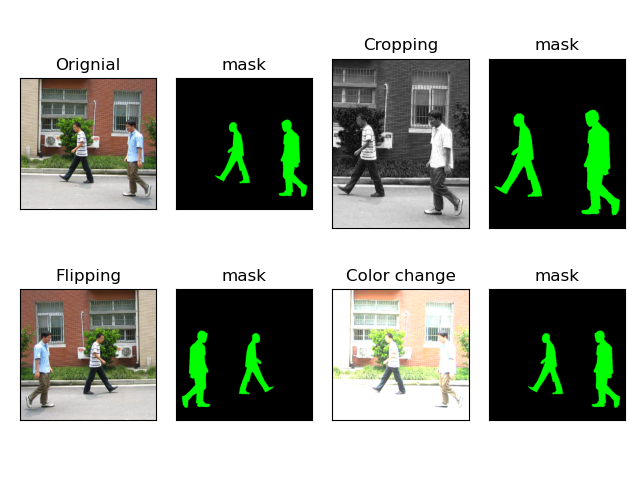
\includegraphics[width=0.5\linewidth]{dataset.png}
	  \caption{Augmentation by cropping, flipping, and colour conversion.}
	  \label{fig:augmentation}
	\end{figure*}

	\par
	It is difficult to drive the CNN model due to the sample sizes are relatively small, some appropriate methods must be used for image augmentation. These methods include resizing, cropping, flipping and colour conversion. The label segmentation mask needs to be modified at the same time while generating new images. Colour conversion using RGB channel separation, blur operation, brightness and contrast adjustment, gamma correction method, etc. Figure \ref{fig:augmentation} shows different methods for image augmentation and the corresponding results. The number of images is expanded to 34680 from only 170 after using the above methods.

%%%%%%%%%%%%%%%%%%%  Section 4 Training and Result analyses%%%%%%%%%%%%%%%%%%
	\section{Training and Result analyses } \justify
	
%	\begin{wrapfigure}{l}{0.7\linewidth}
%	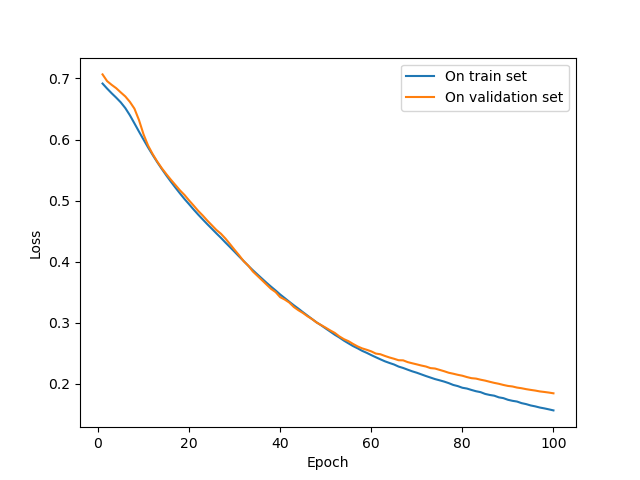
\includegraphics[width=\linewidth]{Figure_1.png}
%	\caption{This is the former Share\LaTeX{} logo}
%	\end{wrapfigure}
	
	\lipsum[1-3]
	\begin{figure*}[htb] %[h!]
	  \centering
	  \begin{subfigure}[b]{0.3\linewidth}
	    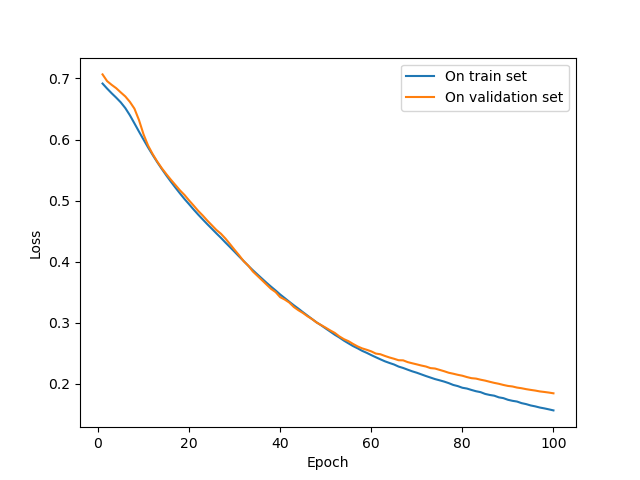
\includegraphics[width=\linewidth]{Figure_1.png}
	    \caption{Loss.}
	  \end{subfigure}
	  \begin{subfigure}[b]{0.3\linewidth}
	    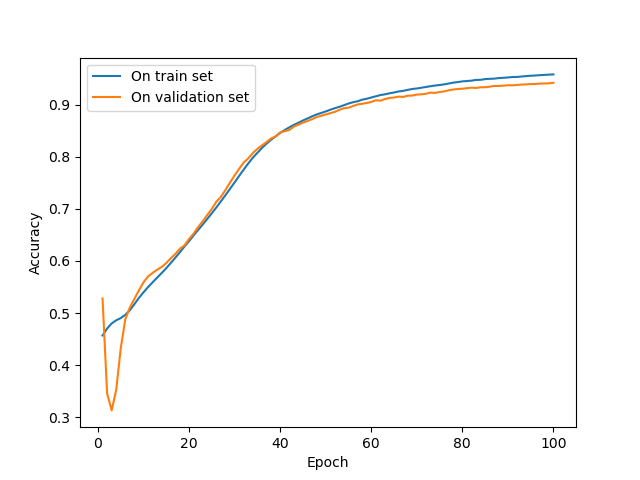
\includegraphics[width=\linewidth]{Figure_2.png}
	    \caption{Accuracy.}
	  \end{subfigure}
	  \caption{Loss and accuracy of the first 100 epochs.}
	  \label{fig:training}
	\end{figure*}
	\lipsum[4]

	The experiment was developed in python and OpenCV-python library and the model trained on Google Collaboratory (GPU). The augmented dataset is divided into two parts before training, 70 percent of them is the training set, and the rest is the test set. Accuracy measurement uses intersection over union (IOU). Figure \ref{fig:training} shows the loss and accuracy of the first 100 epochs on the training set and the test set respectively. After thousands of epochs, loss on the training set are reached -0.2689 and the accuracy reached to 0.8978. Figure \ref{fig:result1} and Figure \ref{fig:result2} respectively demonstrates the pedestrian segmentation effect on different images.
	\lipsum[1-3]
	\begin{figure*}[htb] %[h!]
	  \centering
	  \begin{subfigure}[b]{0.45\linewidth}
	    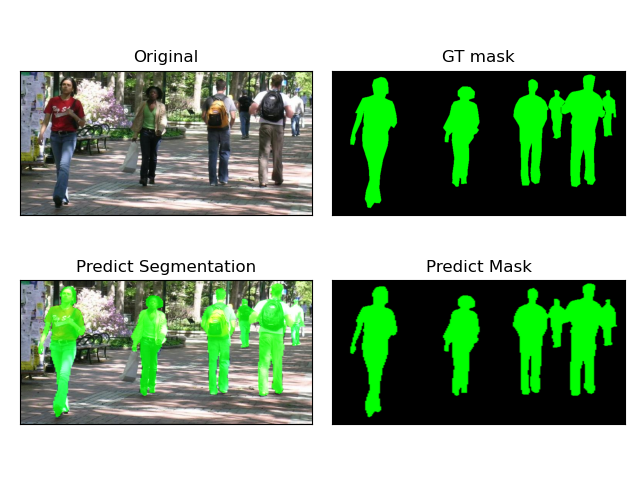
\includegraphics[width=\linewidth]{predictMask1.png}
	    %\caption{}
	  \end{subfigure}
	  \begin{subfigure}[b]{0.45\linewidth}
	    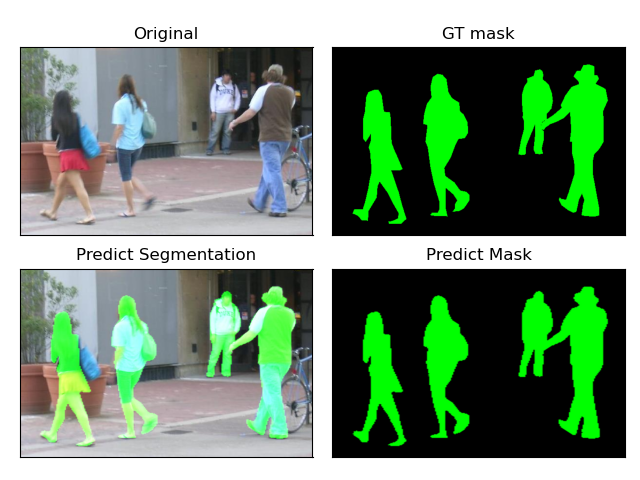
\includegraphics[width=\linewidth]{predictMask2.png}
	    %\caption{}
	  \end{subfigure}
	  \caption{Detection effect of images form dataset.}
	  \label{fig:result1}
	\end{figure*}
	\lipsum[4]

	\lipsum[1-3]
	\begin{figure*}[htb] %[h!]
	  \centering
	  \begin{subfigure}[b]{0.45\linewidth}
	    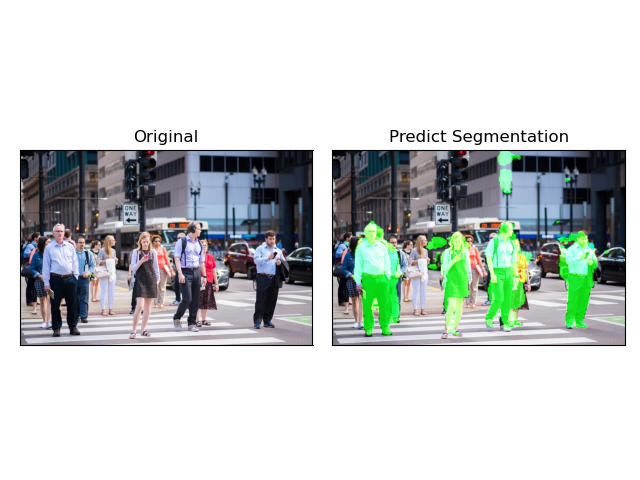
\includegraphics[width=\linewidth]{predict1.png}
	    %\caption{}
	  \end{subfigure}
	  \begin{subfigure}[b]{0.45\linewidth}
	    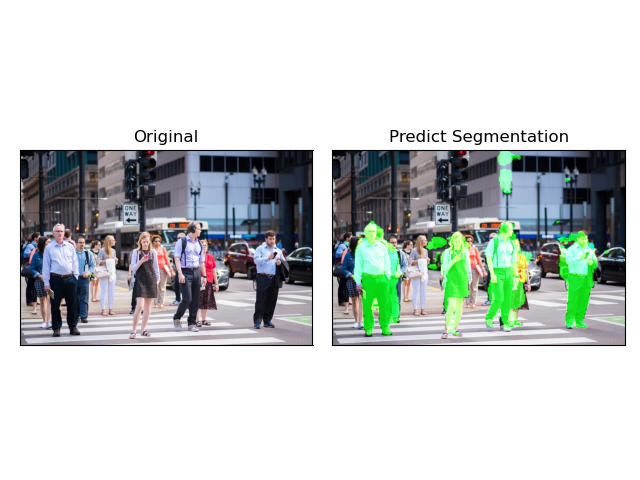
\includegraphics[width=\linewidth]{predict1.png}
	    %\caption{}
	  \end{subfigure}
	  \caption{Detection effect of images not in dataset.}
	  \label{fig:result2}
	\end{figure*}
	\lipsum[4]

%%%%%%%%%%%%%%%%%%%  Section 5 Conclusion %%%%%%%%%%%%%%%%%%%%%%%%%%
	\section{Conclusion} \justify
	According to the results of the experiment, 1) Segmentation for small pedestrians and overlapping pedestrians is not good. 2) The segmentation effect on images with very different scenes from the training samples is poor. The experimental results show that U-Net is effective in pedestrian segmentation tasks. However, due to the limitations of training time and hardware capabilities, the segmentation accuracy has room for further improvement. In addition, the training samples' scene of the dataset is all college students around the university, which may limit the versatility and robustness of the model.

%%%%%%%%%%%%%%%%%%%  References %%%% %%%%%%%%%%%%%%%%%%%%%%%%%%
	%\newpage
	\pagenumbering{gobble}
	\bibliography{comp820}
	\bibliographystyle{ieeetr}  
	%\bibliographystyle{apalike}
	%\setlength{\bibsep}{0.0pt}
	
%%	\let\oldthebibliography\thebibliography
%%	\let\endoldthebibliography\endthebibliography
%%	\renewenvironment{thebibliography}[1]
%%	{
%% 	 \begin{oldthebibliography}{#1}
%%    		\setlength{\itemsep}{10.0em}
%%    		\setlength{\parskip}{10em}
%%	}{  \end{oldthebibliography} 
%%	}

	\end{multicols}
\end{document}